% !TeX encoding = UTF-8
% !TeX program = xelatex
% !TeX spellcheck = en_US

\documentclass[degree=project,degree-type=project,cjk-font=noto]{thuthesis}
\usepackage{mathtools}
\usepackage{tikz}
\usetikzlibrary{shapes,arrows}
\usepackage[autosize]{dot2texi}
% Syntax Highlighting in LaTeX, need pygments
% Must build with xelatex -shell-escape -enable-8bit-chars.
\usepackage{minted}
% https://tex.stackexchange.com/a/112573
\usepackage{tcolorbox}
\usepackage{etoolbox}
\BeforeBeginEnvironment{minted}{\begin{tcolorbox}}%
\AfterEndEnvironment{minted}{\end{tcolorbox}}%
% color for minted
\definecolor{friendlybg}{HTML}{f0f0f0}


% 论文基本配置,加载宏包等全局配置
\thusetup{
    output = electronic,
    title  = {实验二},
    author  = {肖文韬},
    studentid = {2020214245},
    major = {电子信息(计算机技术)},
    email = {xwt20@mails.tsinghua.edu.cn},
    course = {密码学与网络安全},
    include-spine = false,
}


\usepackage{float}
\usepackage[sort]{natbib}
\bibliographystyle{thuthesis-numeric}
\graphicspath{{figures/}}


\setlist[enumerate,1]{label=\arabic*.}
\setlist[enumerate,2]{label=(\alph*)}
\setlist[enumerate,3]{label=\roman*.}
\setlist[enumerate,4]{label=\greek*}

\newcommand*\justify{%
  \fontdimen2\font=0.4em% interword space
  \fontdimen3\font=0.2em% interword stretch
  \fontdimen4\font=0.1em% interword shrink
  \fontdimen7\font=0.1em% extra space
  \hyphenchar\font=`\-% allowing hyphenation
}

\renewcommand{\texttt}[1]{%
  \begingroup
  \ttfamily
  \begingroup\lccode`~=`/\lowercase{\endgroup\def~}{/\discretionary{}{}{}}%
  \begingroup\lccode`~=`[\lowercase{\endgroup\def~}{[\discretionary{}{}{}}%
  \begingroup\lccode`~=`.\lowercase{\endgroup\def~}{.\discretionary{}{}{}}%
  \catcode`/=\active\catcode`[=\active\catcode`.=\active
  \justify\scantokens{#1\noexpand}%
  \endgroup
}


\begin{document}

% 封面
\maketitle

\frontmatter
% % !TeX root = ../thuthesis-example.tex

% 中英文摘要和关键字

\begin{abstract}
  论文的摘要是对论文研究内容和成果的高度概括。摘要应对论文所研究的问题及其研究目
  的进行描述,对研究方法和过程进行简单介绍,对研究成果和所得结论进行概括。摘要应
  具有独立性和自明性,其内容应包含与论文全文同等量的主要信息。使读者即使不阅读全
  文,通过摘要就能了解论文的总体内容和主要成果。

  论文摘要的书写应力求精确、简明。切忌写成对论文书写内容进行提要的形式,尤其要避
  免“第 1 章……;第 2 章……;……”这种或类似的陈述方式。

  本文介绍清华大学论文模板 \thuthesis{} 的使用方法。本模板符合学校的本科、硕士、
  博士论文格式要求。

  本文的创新点主要有:
  \begin{itemize}
    \item 用例子来解释模板的使用方法;
    \item 用废话来填充无关紧要的部分;
    \item 一边学习摸索一边编写新代码。
  \end{itemize}

  关键词是为了文献标引工作、用以表示全文主要内容信息的单词或术语。关键词不超过 5
  个,每个关键词中间用分号分隔。(模板作者注:关键词分隔符不用考虑,模板会自动处
  理。英文关键词同理。)

  % 关键词用“英文逗号”分隔
  \thusetup{
    keywords = {TeX, LaTeX, CJK, 模板, 论文},
  }
\end{abstract}

\begin{abstract*}
  An abstract of a dissertation is a summary and extraction of research work
  and contributions. Included in an abstract should be description of research
  topic and research objective, brief introduction to methodology and research
  process, and summarization of conclusion and contributions of the
  research. An abstract should be characterized by independence and clarity and
  carry identical information with the dissertation. It should be such that the
  general idea and major contributions of the dissertation are conveyed without
  reading the dissertation.

  An abstract should be concise and to the point. It is a misunderstanding to
  make an abstract an outline of the dissertation and words ``the first
  chapter'', ``the second chapter'' and the like should be avoided in the
  abstract.

  Key words are terms used in a dissertation for indexing, reflecting core
  information of the dissertation. An abstract may contain a maximum of 5 key
  words, with semi-colons used in between to separate one another.

  \thusetup{
    keywords* = {TeX, LaTeX, CJK, template, thesis},
  }
\end{abstract*}


% 目录
% \tableofcontents

% 插图和附表清单
% \listoffiguresandtables
% \listoffigures           % 插图清单

% 正文部分
\mainmatter

\chapter{实验介绍}
RSA加密算法是应用最广泛的公钥加密算法,本次实验实现基于RSA算法的加解密以及数字签名功能,包含以下4种操作:生成密钥对、公钥加密、私钥解密和数字签名。
本次实验中密钥长度为2048比特。
实验使用 Rust 语言实现 RSA-2048 的密钥生成,加密解密,以及数字签名操作。

实验目的:

\begin{enumerate}
    \item 熟悉 RSA 公钥加密算法的思路
    \item 学习 RSA 实现上的技巧
    \item 学习 rust 语言的基本用法
\end{enumerate}

实验平台:

\begin{enumerate}
    \item rust 语言
    \item Arch Linux (不依赖具体操作系统,rust 亦可在 windows/macOS 上使用)
\end{enumerate}

\chapter{实验内容}

\section{生成密钥对}

    密钥对的生成过程包括选取随机数,对随机数进行素性测试,根据素数p和q计算n,随机选择和n的欧拉函数互质的e,计算e的逆元d。
选取的大素数p和q应当满足现有的安全性要求,且至少使用两种不同的算法进行素性测试,请在实验报告中说明你选择参数和算法的安全性以及效率。
选取的e同样应当满足安全性要求,至少使用两种不同的算法进行计算逆元d。

\section{素性测试}

本实现采用了两种最主流的概率素性测试算法:

\begin{enumerate}
  \item \textbf{Miller-Rabin 测试},作为费马定理的扩展,每一轮 MR 测试的伪素数的可能性为 $\frac{1}{4}$,所以 $k$ 轮通过仍然是伪素数的可能性为 $4^{-k}$。复杂度 $O(k \log^2 n)$ ($k$ 为测试轮数)。
  \item \textbf{Baillie–PSW 测试}, 结合了 Miller-Rabin 测试和强 Lucas 概率测试。复杂度为 $O(log^2 n)$,低于 MR 测试。
\end{enumerate}

\subsection{模逆运算}

本实现中素数 p 和 q 均为 2048 位,是目前主流的 RSA-2048 实现,密钥长度符合安全要求。

对于 e 的选择,过小的 e(例如 3)会存在安全问题,同时短比特长度和小的 Hamming 权重能够使得加密的效率更加高,目前 OpenSSL 以及其他实现广泛采用的是 65537 (0x10001).
本实现参考主流实现,e 的选择也是 65537.

d 作为 e 的模 $\phi(n)$ 逆元,因为 n 为 4096 位,所以 d 的强度也能够得到保证。

本实现共有两种模逆的算法实现:

\begin{enumerate}
  \item \textbf{扩展欧几里得算法},算法效率 $O(2 \log_{10}(\phi(n)))$(除法运算)。
  \item \textbf{平方幂算法(binary exponentiation)},算法效率 $O(\log(\phi(n)))$。但是该算法只适用于 $\phi(n)$ 为素数的情况。
\end{enumerate}

代码:

  \begin{minted}[texcomments,tabsize=2,fontsize=\normalsize,style=friendly,bgcolor=friendlybg]{rust}
fn modular_inverse(e: &Integer, phi_n: &Integer, method: &str) {
    if method == "extend_gcd" {
        let mut t = Integer::from(0);
        let mut newt = Integer::from(1);
        let mut r = Integer::from(phi_n);
        let mut newr = Integer::from(e);
        let mut quotient = Integer::new();
        let mut tmp = Integer::new();
        while newr.significant_bits() != 0 {
            quotient.assign(&r / &newr);
            tmp.assign(&quotient * &newt);
            tmp *= -1; tmp += &t; t.assign(&newt);
            newt.assign(&tmp);
            tmp.assign(&quotient * &newr);
            tmp *= -1; tmp += &r; r.assign(&newr);
            newr.assign(&tmp);
        }
        if r > 1 { panic!("e is not invertible!"); }
        if t < 0 { t += phi_n; }
        return t;
    } else if method == "binary_exp" {
        if baillie_psw(phi_n, true) {
            println!("phi_n is prime, use binary_exp");
            return Integer::from((&e).pow_mod_ref(
                    &Integer::from(phi_n - 2), &phi_n).unwrap())
        } else {
            return Integer::from((&e).invert_ref(&phi_n).unwrap());
        }
    }
}
  \end{minted}


\begin{figure}[h]
\centering%
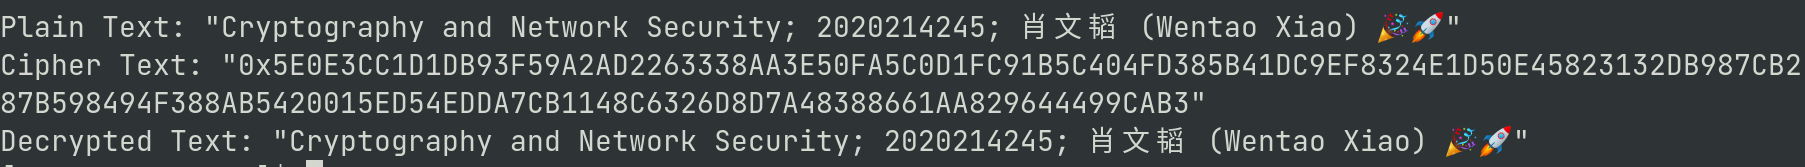
\includegraphics[width=\linewidth]{aes_t4.png}
  \caption{加密机和解密机运行结果}
  \label{fig:t4}
\end{figure}

% 其他部分
\backmatter

% 参考文献
\bibliography{ref/refs}  % 参考文献使用 BibTeX 编译

\end{document}
